\documentclass{article}

% Language setting
% Replace `english' with e.g. `spanish' to change the document language
\usepackage[english]{babel}

% Set page size and margins
% Replace `letterpaper' with`a4paper' for UK/EU standard size
\usepackage[letterpaper,top=2cm,bottom=2cm,left=3cm,right=3cm,marginparwidth=1.75cm]{geometry}

% Useful packages
\usepackage{amsmath}
\usepackage{graphicx}
\usepackage[colorlinks=true, allcolors=blue]{hyperref}

\title{CPE301L: Lab 6}
\author{Joshua Knight, Nicky Victoriano}

\begin{document}
\maketitle
 
\section{Introduction}

In this lab, we are responsible for programming an Arduino to echo the value of a pressed keyboard input into the terminal using register-level programming. In Part 1, it will echo the exact input from the keyboard. In Part 2, it will echo the ASCII code of the input.

\section{Results}

\subsection{Code}

\subsubsection{Part 1: echo2c.ino}

This first section was fairly straightforward. We were provided code in the instructions that outlined the program requirements. The program initializes and sets the memory addresses for each register. Then, it waits for the register to contain a character (and the RDA bit is full), gets the character from the correct memory address, and then outputs the character to the serial monitor when it can (and the TBE bit is empty). The result of this can be seen in \textbf{Figure \ref{fig:echo2c}}. 

\begin{figure}[h!]
\centering
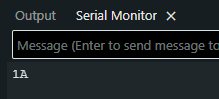
\includegraphics[width=0.5\textwidth]{echo2c.png}
\caption{\label{fig:echo2c}The result of hitting '1' then enter and 'A' then enter.}
\end{figure}

\subsubsection{Part 2: echo3c.ino}

This second section involves outputting hex in the format '0xYY$\backslash$n'. To do this, we heavily used our previously created output character function and created a new function for ease. First, we modified our loop to output our new format (U0putchar('0'), U0putchar('x'), U0putchar('$\backslash$n'), etc.). Then, we added a function that takes 4 bits and converts them to hex. It checks to see if their value is less than 10 to assign digits or letters based on ASCII values. The result of this can be seen in \textbf{Figure \ref{fig:echo3c}}. 

\begin{figure}[h!]
\centering
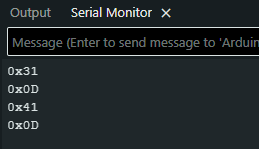
\includegraphics[width=0.5\textwidth]{echo3c.png}
\caption{\label{fig:echo3c}The result of hitting '1' then enter and 'A' then enter, now outputting hex.}
\end{figure}
 
View the code on \href{https://github.com/jrkre/cpe-301}{GitHub}.

\end{document}